% \chapter{Decisões}
\chapter{Trabalhos Relacionados}
% OU \chapter{Engenharia de Software}
% OU \chapter{Tecnologias e Ferramentas Utilizadas}
\label{chap:relacionados}

\section{Introdução}
\label{chap2:sec:intro}
Este capítulo pretende mostrar e comparar algum trabalho já feito anteriormente, na mesma área que o TankUP, de maneira a esclarecer como e onde este se encaixa no ambiente existente. Neste sentido, primeiro é feito um \textit{overview} das características mais gerais do trabalho que foi feito, sendo depois comparado com alguns trabalhos relacionados.

\section{Resumo de Características Gerais}
\label{chap2:sec:DGL}
A seguir, é apresentada uma tabela que resume as características mais gerais da aplicação desenvolvida:
\begin{table}
\caption{Tabela de características gerais.}
\label{tab:tabela_caracteristicas_gerais}
\centering
\begin{tabular}{|c||l|l|}
\hline
\hline
\textbf{\#} & \textbf{Tecnologia} & \textbf{Escolha} \\
\hline
\hline
1 & Plataforma Móvel & \emph{Android} \\
\hline	
2 & Motor de Jogo & Unity3D \\
\hline
3 & Modelação 3D  & Blender\\
\hline
4 & Base do jogo &  Multi-Jogador por Turnos\\
\hline
5 & Linguagem de Programação & C\#\\
\hline
6 & Modelo de Arquitectura de Comunicação & Cliente - Servidor\\
\hline
7 & Modo de Comunicação & Sockets \ac{TCP}\\
\hline
\end{tabular}

\end{table}
\clearpage

\section{Fundamentação das Características Gerais}
\label{chap2:sec:DEL}
A seguir, vão ser explicadas as escolhas relativas às  características gerais supramencionadas, refletindo o  processo de criação em relação à aplicação.
% * <individuoamaral@gmail.com> 12:18:31 13 May 2017 UTC+0100:
% meter uma estatística de utilização no #1
\begin{enumerate}
\item Uma plataforma móvel que está a mostrar um crescimento exponencial em termos de utilização e público. Trata-se de uma plataforma flexível, sendo reconhecida, assim como o \emph{iOS} da \textit{Apple} [1], como as maiores plataformas de distribuição de jogos, atingindo um público avassalador [10]. Nestes termos, há mais de dois biliões de dispositivos móveis únicos a correr aplicações feitas em \emph{Unity} e tendo uma percentagem de trinta e quatro porcento do mercado de motores de jogo do mundo [17]. Têm-se presenciado inúmeros êxitos inesperados em jogos móveis de pequena dimensão (como é o caso com \textbf{Flappy Bird}), que servem para mostrar que a área tem um crescimento possivelmente exponencial, opinião suportada por outras pesquisas [8] [11] e que nascem várias oportunidades propícias a evolução. A escolha também foi feita devido à experiência  com a plataforma Android, vinda de projetos passados.

\item[2]  O motor de jogo escolhido para desenvolver a aplicação foi o \emph{Unity3D}. Este motor de jogo, além de ser grátis para projetos de pequena envergadura, já deu várias provas de como tem qualidade suficiente para ser utilizado por grandes estúdios de jogos e fazer projetos de sucesso. Poderia ter feito a aplicação utilizando a interface gráfica do Android nativo, no entanto, quis aproximar-me o mais possível do \textit{standard} da indústria. Não tinha qualquer experiência no uso desta ferramenta.

\item[3] A ferramenta de modelação usada para a criação dos \textit{assets} gráficos da aplicação foi o Blender, onde foram feitos os modelos do tanque, do jipe e da artilharia utilizados nos clipes de vídeo. Esta escolha foi feita, mais uma vez, com base no \textit{standard} da indústria [7], sendo uma ferramento profissional de renome, sendo utilizada por vários estúdios de sucesso. Não tinha qualquer experiência no uso desta ferramenta.

\item[4] O jogo consiste em dois tabuleiros 4*4, um para cada jogador, onde cada um vai colocar ao calhas seis peças, sendo que nenhum tem acesso ao tabuleiro do outro e, a única maneira de o adivinhar, é utilizando as respostas do jogo quando um jogador acerta em algo do jogador inimigo. A mecânica do jogo consiste numa batalha, por turnos, entre dois jogadores, na qual o objectivo é destruir o máximo dos veículos do outro jogador.

\item[5] A linguagem de programação escolhida para o projeto foi \emph{C\#} [13]. Mais uma vez, esta escolha foi feita com base no \textit{standard} da indústria. Para trabalhar com o motor de jogo \emph{Unity}, a linguagem de programação tem de ser ou \emph{C\#} ou \emph{JavaScript}. Escolhi \emph{C\#} dado a ter mais experiência em linguagens que entram no mesmo modelo que esta (\emph{Java}) do que com \emph{JavaScript}.

\item[6] Para o modelo de comunicação escolhi usar \emph{Cliente/Servidor}, dado ser o modo para o qual o \emph{Unity} oferece melhor suporte. Também havia interesse em explorar melhor os conceitos que formam a base deste modelo. Os restantes conceitos que foram estudados foram \textit{Bluetooth} [6] e \textit{Peer-to-peer} [3].

\item[7] Para o modo de comunicação, em vez de usar as ferramentas disponibilizadas pelo \emph{Unity}, tais como o seu \emph{NetClient} e módulo multijogador, foram utilizados \emph{Sockets \ac{TCP}} [12], dado que assim é possível aperceber-se, de uma forma mais detalhada, como a comunicação entre os clientes e o servidor é feita e qual a dimensão de dados que é preciso passar entre eles.
\end{enumerate}
\clearpage

\section{Projetos Relacionados}
\label{chap2:sec:PRL}
Para a planificação da aplicação, foram considerados dois projetos nos quais me baseei para, de uma maneira mais informada, me ambientar à elaboração da minha aplicação. Estes trabalhos foram: 
\begin{enumerate}
    \item \textbf{Battleship}\\
    De uma forma resumida, o jogo da Batalha Naval [2] consiste num jogo por turnos no qual dois jogadores colocam um determinado número de peças, de vários tipos, no seu tabuleiro sem o conhecimento do outro jogador.
    A cada turno, um jogador seleciona uma posição do tabuleiro do seu adversário para atacar e, caso acerte, tem de lhe ser comunicado por parte do adversário. O jogador que conseguir acertar mais vezes, ganha.

    O clássico jogo da batalha naval, onde existem dois jogadores que colocam um número limitado de peças num tabuleiro, serviu para formar a ideia de jogabilidade fundamental desta aplicação. Toda a mecânica de jogo foi aproveitada deste clássico jogo de tabuleiro, sendo que o que foi mudado foi a ideia de design (jogo de veículos terrestres em vez de navais).

\begin{figure}[!h]
  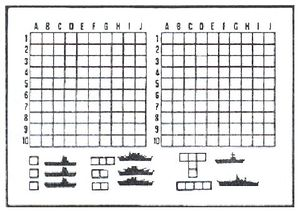
\includegraphics[width=7cm, height=5cm]{Batalhanaval.jpg}
  \centering
  \caption{Clássico Batalha Naval.}
  \label{fig:batalhanaval}
\end{figure}
   
    
    \item \textbf{Clash Royale}\\
    Um jogo [14] que pouco tem em comum com a aplicação desenvolvida, mas que serviu de inspiração para o design e a sua filosofia. O jogo consiste em dois jogadores que têm um exército ao seu dispôr e numa arena, onde estes lutam, dando ordens aos seus exércitos para atacar o outro jogador.
    Neste caso, o jogador tem de escolher a posição onde colocar as suas tropas, sendo que este facto se torna muito importante na mecânica de jogo. 

    A ideia de utilizar um tabuleiro geral para ambos os jogadores, apenas desenhando os \textit{assets} necessários para que cada um veja apenas o necessário em cada momento, veio da interação dos menus do jogo com a mecânica de jogo em si.

\begin{figure}[!h]
  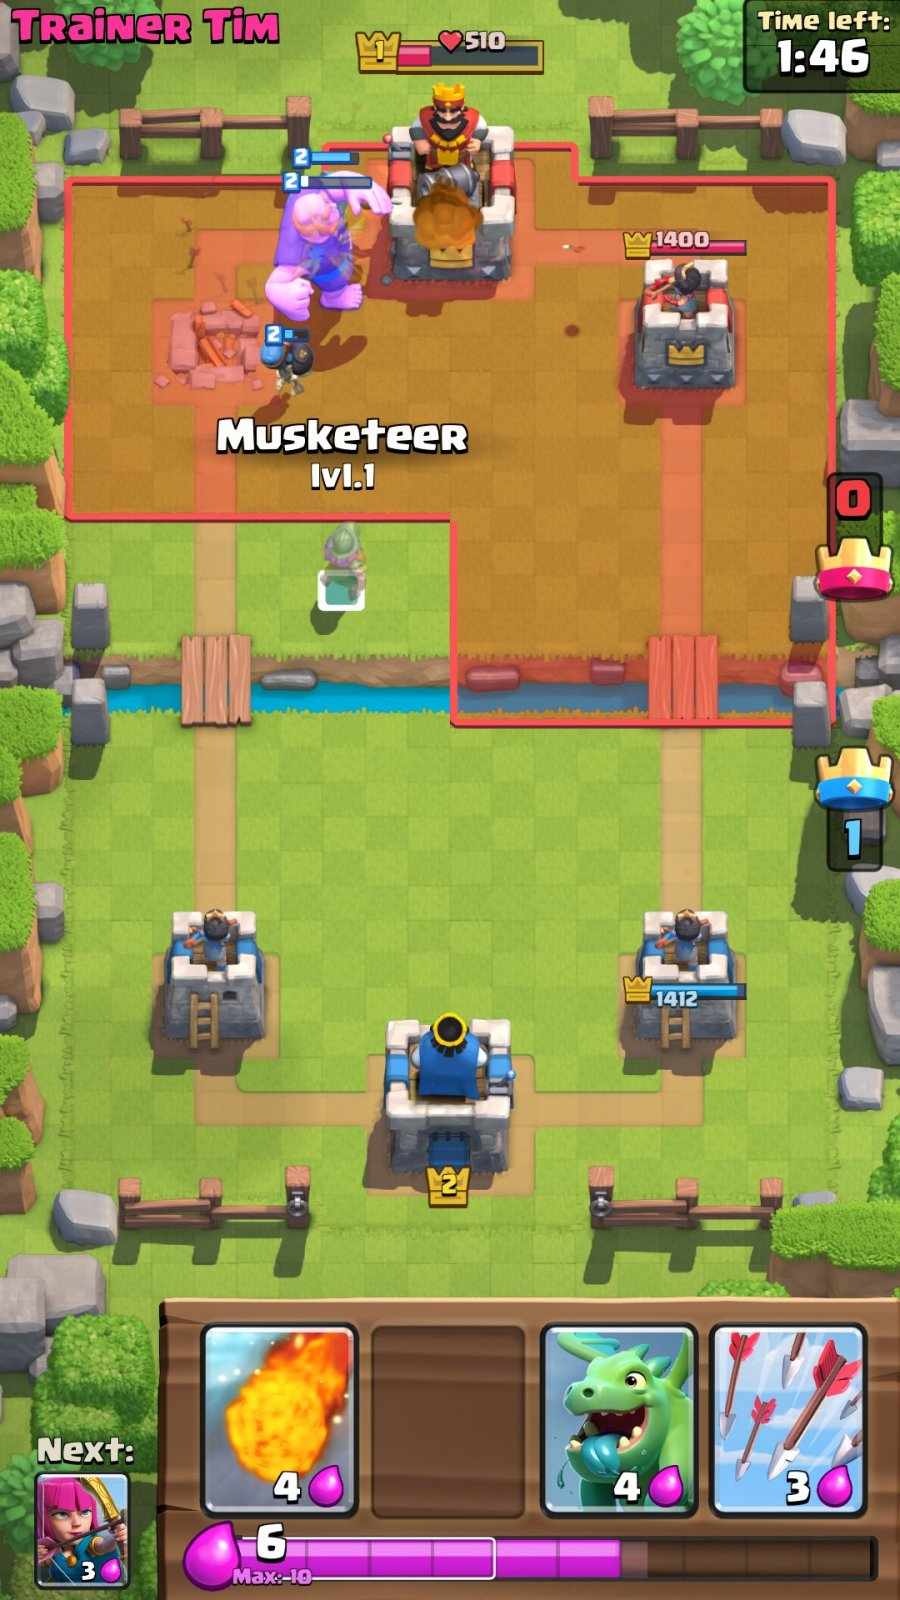
\includegraphics[width=10cm, height=11cm]{clash-royale-4.jpg}
  \centering
  \caption{Ecrã de jogo de uma partida de Clash Royale.}
  \label{fig:clash}
\end{figure}

\end{enumerate}



\clearpage
\section{Conclusões}
\label{chap2:sec:conc}
Com este capítulo, são explicadas as ideias tidas no decorrer do desenvolvimento da aplicação, transmitindo assim uma ideia geral do \textit{mindset} e as bases que foram utilizadas para construir a aplicação. Partindo desta informação, é agora possível avançar para o capítulo referente às \textbf{tecnologias e ferramentas utilizadas} \autoref{chap:tecnologias_ferramentas_utilizadas} no desenvolvimento da aplicação.